\part{Engineering and Execution}

\chapter{The host, the data path, and the training stack}
\label{r:ch:host}

\section{The host and its constraints}

All Study~2 and Amendment~8 computation ran on one shared server (\texttt{node1}) with eight NVIDIA RTX A6000 GPUs
(49~GB each). It has no job scheduler; work runs directly on the login node. The operating rules for the project were:
never more than four GPUs at once, check for vacant GPUs first, keep data that feeds GPUs off the shared network
filesystem, use the fast local disk and vacate it afterwards.

\begin{longtable}{p{0.26\textwidth}p{0.64\textwidth}}
\caption{Host constraints discovered or imposed, and the response to each.}\label{r:tab:host}\\
\toprule
Constraint & Consequence and response \\
\midrule
\endfirsthead
\toprule
Constraint & Consequence and response \\
\midrule
\endhead
\bottomrule
\endfoot
Four GPUs at most & Study~2 used GPUs 0, 3, 4, 5 (GPUs 1 and 2 were in use by another user); Amendment~8 used 4--7 after
another user started jobs on 0--3 twenty-five minutes before launch. The scheduler refuses more than four. \\
Four CPU cores per user & Found during Study~2 preparation: the per-user cgroup quota is 400\% (four cores) on a
128-core machine. The power simulation ran far slower than its core count suggested, a data-loader benchmark was invalid,
and per-image augmentation in loader workers could not feed even one GPU. This is very likely the ``host bottleneck''
recorded in Study~1 (Chapter~\ref{s1:ch:ch13_execution_lifecycle_failures_and_demotiv}). Response: decode crops once into
caches, upload them to the GPU, augment there (Section~\ref{r:ch:gpuaug}), keep CPU threads low, and run heavy CPU
analyses on a workstation. \\
\texttt{/scratch} not writable & All node-local work used \texttt{/tmp/rchethan1\_cytofair} (the 192~GB root partition
shared with the operating system) and \texttt{/dev/shm}; a disk guard keeps 40~GB free. \\
Slow network home & The NFS home can stall under load; a recursive search over it had to be stopped early in Study~2
preparation. Rule adopted: only static artifacts go there, and copies are single bandwidth-limited streams. \\
Shared GPUs & Other users' jobs can appear at any time. The scheduler checks each GPU's memory before launching
(at most 30,000~MiB in use), and an infrastructure failure caused by another process does not count as a retry
(Amendment~7). \\
No scheduler & Background controllers launched with \texttt{setsid nohup} and detached from the SSH session; a status
file records every running task, completion, and failure. \\
\end{longtable}

\section{The data path}
\label{r:ch:datapath}

\subsection{Provenance to splits}

Every split is derived from the provenance maps of Study~1 (\artifact{provenance/*.parquet}), whose recovery and
verification are described in Part~II. \texttt{cytofair study2-design} writes every Study~2 split, factorial design,
transplant plan, and the probe split with SHA-256 hashes into \artifact{splits/study2/study2_split_manifest.csv};
\texttt{cytofair followup-design} does the same for Amendment~8 (\artifact{splits/study2/followup/}). Trainers hash the
split file before use and refuse a mismatch.

\subsection{Packed crop caches}

Decoding thousands of small BMP and PNG files on four cores is slow, and reading them from the network home is
unreliable. Each image set is therefore packed once into a cache on the node-local disk: one \texttt{uint8} array of all
pixels (\texttt{\{name\}\_pixels.npy}, memory-mapped), an index (\texttt{\{name\}\_index.parquet}) with each crop's offset,
height, width, and the SHA-256 of its pixels, and a manifest with the SHA-256 of both files. A cache is verified on load;
a hash mismatch stops the run.

\begin{longtable}{p{0.3\textwidth}p{0.18\textwidth}p{0.45\textwidth}}
\caption{Caches used by Study 2 and Amendment 8 (hashes in Appendix~\ref{r:app:hashes}).}\label{r:tab:caches}\\
\toprule
Cache & Images & Content \\
\midrule
\endfirsthead
\bottomrule
\endfoot
\texttt{sipakmed} & 4,049 & every SIPaKMeD crop \\
\texttt{cric} & 11,534 & $100\times100$ windows around every CRIC nucleus \\
\texttt{transplant\_seed*} (10) & 4,096--4,400 each & 2B composites of each seed's common test set \\
\texttt{sipakmed\_masked} & 4,049 & background set to the ImageNet mean (F3) \\
\texttt{sipakmed\_reinhard50/100} & 4,049 each & Reinhard normalisation at strength 0.5 and 1 (F6) \\
\texttt{ablation\_seed*} (10) & six per test crop & the F2 carrier ablations \\
\end{longtable}

\section{The GPU-resident input path}
\label{r:ch:gpuaug}

\begin{figure}[H]
\centering
\begin{adjustbox}{max width=\textwidth}
\begin{tikzpicture}[node distance=4mm and 4mm]
\node[box=25mm] (cache) {Packed cache\\\footnotesize uint8, one memmap};
\node[box=25mm, right=of cache] (gpu) {GPU-resident crops\\\footnotesize uploaded once per run};
\node[box=25mm, right=of gpu] (params) {RRC parameters\\\footnotesize CPU generator, exact torchvision port};
\node[box=25mm, right=of params] (crop) {Crop, antialiased resize, flips};
\node[gold=25mm, below=of crop] (color) {Optional HED + BC jitter\\\footnotesize Amendment 8 colour arm};
\node[box=25mm, left=of color] (norm) {ImageNet normalise};
\node[box=25mm, left=of norm] (model) {Backbone + head\\\footnotesize deterministic kernels};
\node[box=25mm, left=of model] (out) {Logits, features, weights};
\draw[flow] (cache) -- (gpu); \draw[flow] (gpu) -- (params); \draw[flow] (params) -- (crop);
\draw[flow] (crop) -- (color); \draw[flow] (color) -- (norm); \draw[flow] (norm) -- (model); \draw[flow] (model) -- (out);
\end{tikzpicture}
\end{adjustbox}
\caption{The GPU-resident training input path. The host allowed four CPU cores per user, which made per-image PIL
augmentation in data-loader workers the bottleneck; moving the registered augmentation onto the GPU removed it
while sampling exactly the same crop geometry as torchvision for the same random stream.}
\label{r:fig:gpu-augment}
\end{figure}


The registered augmentation is \texttt{RandomResizedCrop(224, scale 0.8--1.0, ratio 3/4--4/3)}, horizontal and vertical
flips, and ImageNet normalisation. \artifact{src/cytofair/gpu_augment.py} keeps every crop of a split on the GPU as a
\texttt{uint8} tensor and draws crop parameters with an exact port of torchvision's \texttt{RandomResizedCrop.get\_params}
from an explicit CPU generator, including the float32 exponential torchvision uses for the aspect ratio. A unit test
compares the sampled geometry with torchvision's for four image shapes and 25 seeds each and requires identity. Resizing
uses antialiased bilinear interpolation, PyTorch's implementation of PIL's filter, which can differ from PIL by uint8
rounding. The Amendment~8 colour arm adds HED optical-density jitter and brightness/contrast jitter, drawn from the same
generator after the geometry, so runs without colour augmentation reproduce the registered random stream exactly.

\section{Determinism}
\label{r:ch:determinism}

Every run sets cuDNN deterministic mode, disables cuDNN benchmarking, calls
\path{torch.use_deterministic_algorithms(True, warn_only=True)}, and sets \texttt{CUBLAS\_WORKSPACE\_CONFIG=:4096:8}.
During smoke tests ViT-B/16 raised a warning that the memory-efficient attention backward pass is non-deterministic; the
flash, memory-efficient, and cuDNN attention kernels were disabled in favour of the math kernel, and two identical ViT
runs then produced bitwise-identical logits. The follow-up evaluation code avoids \texttt{index\_add\_} (non-deterministic
on CUDA) by computing group sums as one-hot matrix products.

Final weights are stored in float16 to halve their size. Re-evaluating the saved Phase~1 checkpoints reproduced the
recorded test accuracy exactly for 418 of 480 models; 56 differed by one test crop and six by two or three crops out of
810, all from float16 rounding. Every follow-up comparison is made within one re-evaluation, so this does not bias any
registered contrast.

\section{What every run leaves behind}
\label{r:ch:artifacts}

\artifact{src/cytofair/train_study2.py} writes, for every run:
\begin{itemize}[leftmargin=1.6em]
\item a JSON record with the dataset, protocol, architecture, seed, accuracy, macro-F1, balanced accuracy, NLL, 15-bin ECE,
the confusion matrix, train and test crop and parent counts, the fraction of test crops with a training parent, the
recipe and augmentation, adversary settings, the split file and semantic hashes, cache hashes, the git commit, GPU,
start and end times, runtime metadata, a per-epoch history, and the path and SHA-256 of every artifact;
\item per-crop test logits (Parquet), float16 final weights, penultimate features of the 1,696 probe crops (NPZ), and
logits for any registered extra evaluation set (the 2B composites).
\end{itemize}
The follow-up evaluation tasks write comparable records (\artifact{src/cytofair/followup_eval.py}), verifying each
checkpoint's hash before loading it. The exported tables in \artifact{results/study2/run_records} keep every field the
record plots, including all \RecEpochs\ epoch histories.

\chapter{Scheduling, execution, and archiving}
\label{r:ch:scheduler}

\section{Scheduling, failure handling, and collection}

\begin{figure}[H]
\centering
\begin{adjustbox}{max width=\textwidth}
\begin{tikzpicture}[node distance=5mm and 7mm]
\node[box=28mm] (pending) {Pending\\\footnotesize sorted by priority, file order};
\node[box=28mm, right=of pending] (guard) {Guards\\\footnotesize free disk $\geq$ 40 GB, GPU memory, slot units};
\node[box=28mm, right=of guard] (running) {Running\\\footnotesize one GPU per training task, two per evaluation task};
\node[done=28mm, below=of running] (done) {Completed\\\footnotesize result JSON + artifacts exist};
\node[gold=28mm, left=of done] (retry) {Retry once\\\footnotesize same seed, split, code};
\node[bad=28mm, left=of retry] (fail) {Failed\\\footnotesize recorded; analysis fails closed};
\draw[flow] (pending) -- (guard); \draw[flow] (guard) -- (running);
\draw[flow] (running) -- node[note, right]{rc 0 and valid} (done);
\draw[flow] (running) -- node[note, above, sloped]{error} (retry);
\draw[flow] (retry) -- node[note, above]{second error} (fail);
\draw[flow] (retry.north) to[bend left=20] (pending.south east);
\end{tikzpicture}
\end{adjustbox}
\caption{The resumable scheduler (\texttt{scripts/\allowbreak study2/\allowbreak launch\_matrix.py}). A task whose valid result already exists is
skipped on restart, so the controller can be relaunched after any interruption without duplicating a run.}
\label{r:fig:launcher}
\end{figure}


A task is a JSON line naming its command, the result file that proves completion, a priority, the GPU share it needs,
and an \texttt{expect} block of fields its result must carry (dataset, protocol, architecture, seed, split hash, and for
the follow-up arms the cache, colour augmentation, and adversary). \artifact{scripts/study2/build_tasks.py} wrote the
1,341 Study~2 tasks and \artifact{scripts/study2/build_followup_tasks.py} the 1,580 follow-up tasks; both sets are
committed and hashed. Training tasks took a whole GPU; evaluation-only tasks took half, so two ran per GPU.

The collectors (\artifact{analysis/study2/collect_runs.py}, \artifact{analysis/study2/followup/prepare_followup.py})
require exactly one valid result per registered task whose recorded fields match its \texttt{expect} block; anything
missing, duplicated, or mismatched is listed and the analysis stops. \texttt{--allow-incomplete} produces progress reports
only. Under Amendment~7, adversarial runs whose every attempt ended in a non-finite loss are recognised from their logs and
recorded as diverged rather than missing. Neither matrix had a failure, retry, or divergence.

\section{Execution}
\label{r:ch:execution}

\subsection{Smoke tests}

Before each registration, short runs exercised every code path on splits that cannot reveal a registered contrast: P1
splits only for Study~2; leak cells, single P1 runs, and single evaluation tasks for Amendment~8
(Table~\ref{r:tab:ledger-smoke}). Their metrics were checked only for finiteness and integrity (for example, that a
re-evaluated checkpoint reproduces its recorded accuracy).

\subsection{The two matrices}

\begin{figure}[H]
\centering
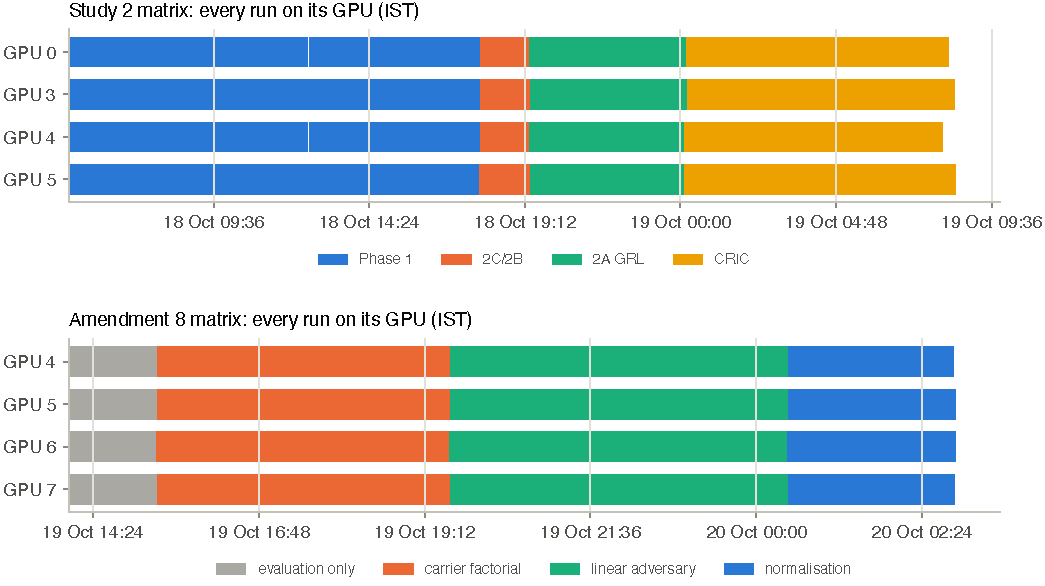
\includegraphics[width=\textwidth]{gpu_schedule.pdf}
\caption{Every run of both matrices on its GPU, from the start and end times in the run records (evaluation tasks from
the controller log). The arms ran in priority order; white gaps are launch overhead.}
\label{r:fig:gpu-schedule}
\end{figure}

{\footnotesize
\setlength{\tabcolsep}{3.5pt}
\begin{longtable}{lrrrll}
\caption{Compute ledger of every Study 2 and Amendment 8 arm (node1, NVIDIA RTX A6000; times in IST). GPU-hours are summed per-run elapsed time; runs shared four GPUs.}\label{r:tab:compute}\\
\toprule
Arm & Runs & Mean min & GPU-h & First start & Last finish \\
\midrule
\endfirsthead
\toprule
Arm & Runs & Mean min & GPU-h & First start & Last finish \\
\midrule
\endhead
\bottomrule
\endfoot
Study 2 Phase 1 (H1) & 720 & 3.9 & 47.1 & 18 Oct 05:07 & 18 Oct 17:50 \\
Study 2 2C/2B (H3, H4) & 160 & 2.0 & 5.4 & 18 Oct 17:48 & 18 Oct 19:21 \\
Study 2 2A (H5) & 280 & 3.9 & 18.2 & 18 Oct 19:20 & 19 Oct 00:12 \\
Study 2 CRIC (H2) & 180 & 10.7 & 32.0 & 19 Oct 00:06 & 19 Oct 08:28 \\
A8 carrier factorial (F3, F4) & 480 & 1.9 & 15.2 & 19 Oct 15:19 & 19 Oct 19:34 \\
A8 linear adversary (F7) & 300 & 3.7 & 18.5 & 19 Oct 19:33 & 20 Oct 00:27 \\
A8 stain normalisation (F6) & 160 & 3.4 & 9.1 & 20 Oct 00:27 & 20 Oct 02:52 \\
A8 ablations + Grad-CAM (F2) & 160 & 0.2 & 0.6 & 19 Oct 14:03 & 19 Oct 14:14 \\
A8 LEACE erasure (F5) & 480 & 0.8 & 6.5 & 19 Oct 14:13 & 19 Oct 15:19 \\
\end{longtable}
}


\begin{figure}[H]
\centering
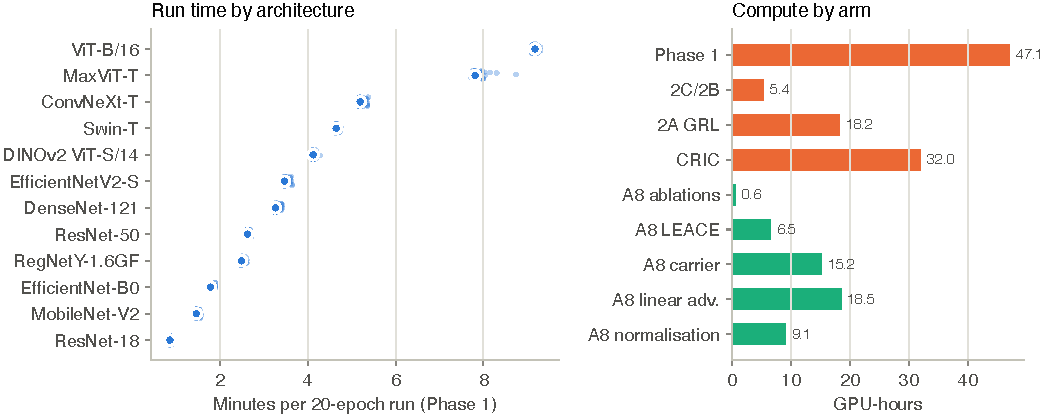
\includegraphics[width=\textwidth]{runtime.pdf}
\caption{Left: wall time of each Phase~1 run by architecture (dots) and its median (ring). Right: GPU-hours by arm.}
\label{r:fig:runtime}
\end{figure}

\subsection{Software}

{\footnotesize
\setlength{\tabcolsep}{3.5pt}
\begin{longtable}{lp{11cm}}
\caption{Software and hardware recorded in every training run.}\label{r:tab:software}\\
\toprule
Component & Version \\
\midrule
\endfirsthead
\toprule
Component & Version \\
\midrule
\endhead
\bottomrule
\endfoot
python & 3.13.9 \\
torch & 2.9.0+cu128 \\
torchvision & 0.24.0+cu128 \\
timm & 1.0.22 \\
cuda & 12.8 \\
cudnn & 91002 \\
cuda\_device & NVIDIA RTX A6000 \\
numpy & 2.5.2 \\
pandas & 3.0.5 \\
scipy & 1.18.1 \\
scikit\_learn & 1.9.0 \\
opencv & 5.0.0 \\
pillow & 12.3.0 \\
platform & Linux-4.18.0-372.9.1.el8.x86\_64-x86\_64-with-glibc2.28 \\
cublas\_workspace\_config & :4096:8 \\
\end{longtable}
}


\section{Archiving and vacating}
\label{r:ch:archive}

\begin{figure}[H]
\centering
\begin{adjustbox}{max width=\textwidth}
\begin{tikzpicture}[node distance=4mm and 5mm]
\node[box=27mm] (local) {Node-local outputs\\\footnotesize /tmp, fast disk};
\node[box=27mm, right=of local] (rsync) {rsync to NFS home\\\footnotesize 20 MB/s, one stream};
\node[box=27mm, right=of rsync] (verify) {Verify\\\footnotesize every size; seeded re-hash sample};
\node[done=27mm, right=of verify] (free) {Free local copy\\\footnotesize only after verification};
\node[gold=27mm, below=of rsync] (hold) {Hold while needed\\\footnotesize Phase 1 and 2C checkpoints until LEACE / ablations finish};
\draw[flow] (local) -- (rsync); \draw[flow] (rsync) -- (verify); \draw[flow] (verify) -- (free);
\draw[flow, dashed] (local) |- (hold); \draw[flow, dashed] (hold) -| (verify);
\end{tikzpicture}
\end{adjustbox}
\caption{Offloading and archiving. The network home is slow and can stall, so copies are single, bandwidth-limited
streams; nothing node-local is deleted until its archived copy has been verified.}
\label{r:fig:archive}
\end{figure}


The follow-up matrix would write about 52~GB of checkpoints into a 71~GB margin, so Study~2 checkpoints were moved to
the network home while it ran: the gradient-reversal and CRIC checkpoints first, then the 2C checkpoints once all 160
ablation tasks had finished, then the Phase~1 checkpoints once all 480 LEACE tasks had finished. Each experiment was
copied, every checkpoint's size compared, a seeded sample of fifty re-hashed against the hash in its run record, and only
then deleted locally. At the end, the follow-up outputs were copied and verified (3,580 artifacts, sizes all matching,
100 re-hashed), the remaining Study~2 outputs re-verified (4,000 artifacts, 200 re-hashed), and the node-local working
directory and shared-memory directory deleted. The archive (\texttt{\textasciitilde/cytofair\_study2\_archive}, 121~GB)
holds every run record, prediction, feature file, checkpoint, log, and status file.

\chapter{Errors, setbacks, and fixes}
\label{r:ch:errors}

Study~1's setbacks (the invalid first classification matrix, the MAnet numerical failure, and the host bottleneck) are
recorded in Chapter~\ref{s1:ch:ch13_execution_lifecycle_failures_and_demotiv}. Everything that went wrong afterwards is
listed here, including mistakes in tooling and in procedure; none changed a registered model, split, seed, or
endpoint.

{\small
\begin{longtable}{p{0.04\textwidth}p{0.26\textwidth}p{0.34\textwidth}p{0.23\textwidth}}
\caption{Every error and setback of Study 2 and Amendment 8, and its fix.}\label{r:tab:errors}\\
\toprule
\# & What went wrong & Fix & Effect on results \\
\midrule
\endfirsthead
\toprule
\# & What went wrong & Fix & Effect on results \\
\midrule
\endhead
\bottomrule
\endfoot
\multicolumn{4}{l}{\textbf{Study 2 preparation (before registration)}} \\
1 & No PDF text tools on the workstation & Python PDF libraries for reading and rendering & none \\
2 & A recursive search over the slow network home stalled & stopped; rule: never scan the network home & none \\
3 & \texttt{/scratch} not writable & node-local \texttt{/tmp} and \texttt{/dev/shm} & none \\
4 & Four-core CPU quota starved data loaders & GPU-resident augmentation; heavy CPU analysis off-host & none (exact port, unit-tested) \\
5 & Power script mis-named variance components; correlation on its $-1$ boundary & pattern matching; correlation set to 0 in the simulation & documented in the plan \\
6 & R: S4 slot read with \texttt{\$} in the protocol model & \texttt{@optinfo} & none \\
7 & R: tidy-evaluation operator inside base \texttt{subset} & explicit indexing & none \\
8 & 2C budget of 240 crops per class infeasible for some seeds & 220 crops, low/high ratio 0.70, feasible for 100/100 seeds & chosen before training \\
9 & pandas 3 read-only arrays; Pillow deprecation & copies; argument removed & none \\
10 & Non-deterministic attention backward (ViT) & math attention kernel only; bitwise repeat verified & none \\
11 & Lint findings, a wrong test expectation & fixed & none \\
12 & SSH launches hung on backgrounded command chains & \texttt{cd; setsid nohup \ldots\ \& disown} & none \\
13 & A shell wait loop did not split its input & explicit \texttt{read} & none \\
14 & No rule for diverged adversarial runs & Amendment~7, before any 2A run & none (no divergence) \\
\multicolumn{4}{l}{\textbf{Study 2 analysis}} \\
15 & One float16 probe-feature row overflowed (EfficientNetV2-S, one crop) & documented; no follow-up arm reads it & one crop in a descriptive measure \\
16 & A completion watcher never fired & replaced with a file-based check & none \\
\multicolumn{4}{l}{\textbf{Amendment 8}} \\
17 & Inference-mode tensors reused in autograd; non-deterministic \texttt{index\_add\_} & clone; one-hot matrix sums & caught in tests \\
18 & R summary object not serialisable to JSON & converted to a list & caught in dry run \\
19 & Remote \texttt{pgrep -f} matched its own command line & file-based completion checks & none \\
20 & Interim preparer crawled on a GPU busy with training & stopped; registered run on a free GPU & none \\
21 & \textbf{Preparer labelled standard carrier runs as colour-augmented} (\texttt{None} became a truthy NaN) & condition read from each run record; unit test; \textbf{Amendment~9} & script halted before output; no estimate seen \\
22 & An archive fetch included smoke checkpoints & refetched records only & none \\
23 & Dose figure plotted out-of-regime levels; labels overlapped & registered regimes only; layout fixed & presentation only \\
24 & Negative numbers typeset with a hyphen & typographic minus in the macro generator & presentation only \\
\end{longtable}
}

\begin{warningbox}{The one that mattered}
Error 21 is the only one that could have changed a reported number. The synthetic dry run had written condition
labels directly and so never exercised the preparer's labelling. The R script stopped at F4 because the contrast term was
missing, which exposed the bug before any output existed. The lesson recorded for the future: dry runs must go through
every stage of the real pipeline, not start from the tables that stage produces.
\end{warningbox}
